%%%%%%%%%%%%%%%%%%%%%%%%
%
% $Autor: Hemanth Jadiswami Prabhakaran $
% $Datum: 2026-09-12 $
% $Pfad: GitHub/MBIDA_Thesis/report/Contents/General/en/04DomainKnowledgeTools.tex $
% $Version: 1 $
%
% $Project: MBIDA Thesis $
%
%%%%%%%%%%%%%%%%%%%%%%%%

\chapter{Domain Knowledge -- Tools}
\label{chap:domainKnowledgeTools}

This chapter describes the Python forecasting ecosystem used to implement the pipeline introduced in Chapter~\ref{chap:methodology}: \texttt{statsforecast} for fitting the base forecasting models, \texttt{hierarchicalforecast} for building the hierarchy and reconciling forecasts across it, \texttt{utilsforecast} for the accuracy metric used throughout this thesis, and the supporting data and visualisation stack (pandas, NumPy, PyArrow, Streamlit, Plotly). Design rationale for why particular models, reconciliation methods, and the sMAPE metric were chosen is covered in Chapter~\ref{chap:methodology} methodology; how these libraries are actually called and configured is covered in Chapter~\ref{chap:appDevelopment} Application Development.

\section{statsforecast}
\label{sec:statsforecastTool}

\texttt{statsforecast} \cite{Garza:2022} is the library used to fit all three base forecasting models used in this thesis -- HistoricAverage, AutoETS, and Theta -- across every series in the hierarchy at once. Rather than looping over series individually, its \texttt{StatsForecast} class accepts a list of model instances and fits them in parallel across the full panel of series in a single call, which is what makes fitting tens of thousands of series computationally practical.

Two configuration options are used throughout the pipeline. First, a \texttt{fallback\_model} (\texttt{HistoricAverage()}) is registered as a safety net: on a panel of this size, some series will be too short, too sparse, or too irregular for ETS or Theta to fit successfully, and rather than the entire run failing on one problematic series, that series is silently given the HistoricAverage forecast instead. How often this fallback actually triggers is a pipeline result, reported in Sections~\ref{sec:testingValidation} and~\ref{sec:testingValidationResults} together with the rest of the testing and validation checks. Second, each model is given a distinct \texttt{alias} (\texttt{histavg}, \texttt{ets}, \texttt{theta}), which becomes both its output column name and part of the naming scheme centralised in \texttt{config.py} (Chapter~\ref{chap:devToDeployment}).

\section{hierarchicalforecast}
\label{sec:hierarchicalforecastTool}

\texttt{hierarchicalforecast} \cite{Olivares:2023} provides the two capabilities that make the hierarchy itself computationally usable: building it, and reconciling forecasts across it.

Its \texttt{aggregate()} function takes the bottom-level (item-store) panel and a specification of the hierarchy's levels, and returns three objects in a single call: \texttt{Y\_df}, the target values rolled up to every level of the hierarchy (not just the bottom); \texttt{S\_df}, the summing matrix -- a compact representation of exactly how bottom-level series roll up into every higher node, stored in sparse form to keep memory use manageable at this scale; and \texttt{tags}, a lookup of which series belong to which hierarchy level, used later when evaluating accuracy separately per level. Because this is built once from a single, already-fixed item universe, the same hierarchy serves the training, test, and live periods without being rebuilt.

Reconciliation itself is performed by a \texttt{HierarchicalReconciliation} object, to which the three reconciliation methods used in this thesis are passed as sparse variants: \texttt{BottomUpSparse} (Section~\ref{subsec:bottomUp}), \texttt{MinTraceSparse} (configured with \texttt{method="wls\_struct"}, the structural weighting scheme derived formally in Section~\ref{subsec:minTrace}, and \texttt{nonnegative=True}, enforcing the constraint motivated in Section~\ref{sec:clippingRationale}), and \texttt{TopDownSparse} (configured with \texttt{method="proportion\_averages"}, the historical-share disaggregation described in Section~\ref{subsec:topDown}). The library also supplies an \texttt{evaluate()} function that computes sMAPE per series and averages the result within each hierarchy level, which is what produces the by-level accuracy tables used in Chapter~\ref{chap:evaluation}.

Figure~\ref{fig:toolDataFlow} summarises how the three Nixtla libraries introduced in this and the next section hand data to one another: \texttt{aggregate()} builds the hierarchy once, \texttt{StatsForecast} fits every series against the resulting panel, \texttt{HierarchicalReconciliation} combines the base forecasts with the hierarchy's own structure to produce coherent forecasts, and \texttt{evaluate()} scores the result. This is a narrower, tool-level view than the full pipeline diagram in Chapter~\ref{chap:appDevelopment} (Figure~\ref{fig:pipelineFlow}): it shows which library is responsible for which data object, not every processing step in between.

\begin{figure}[H]
	\centering
	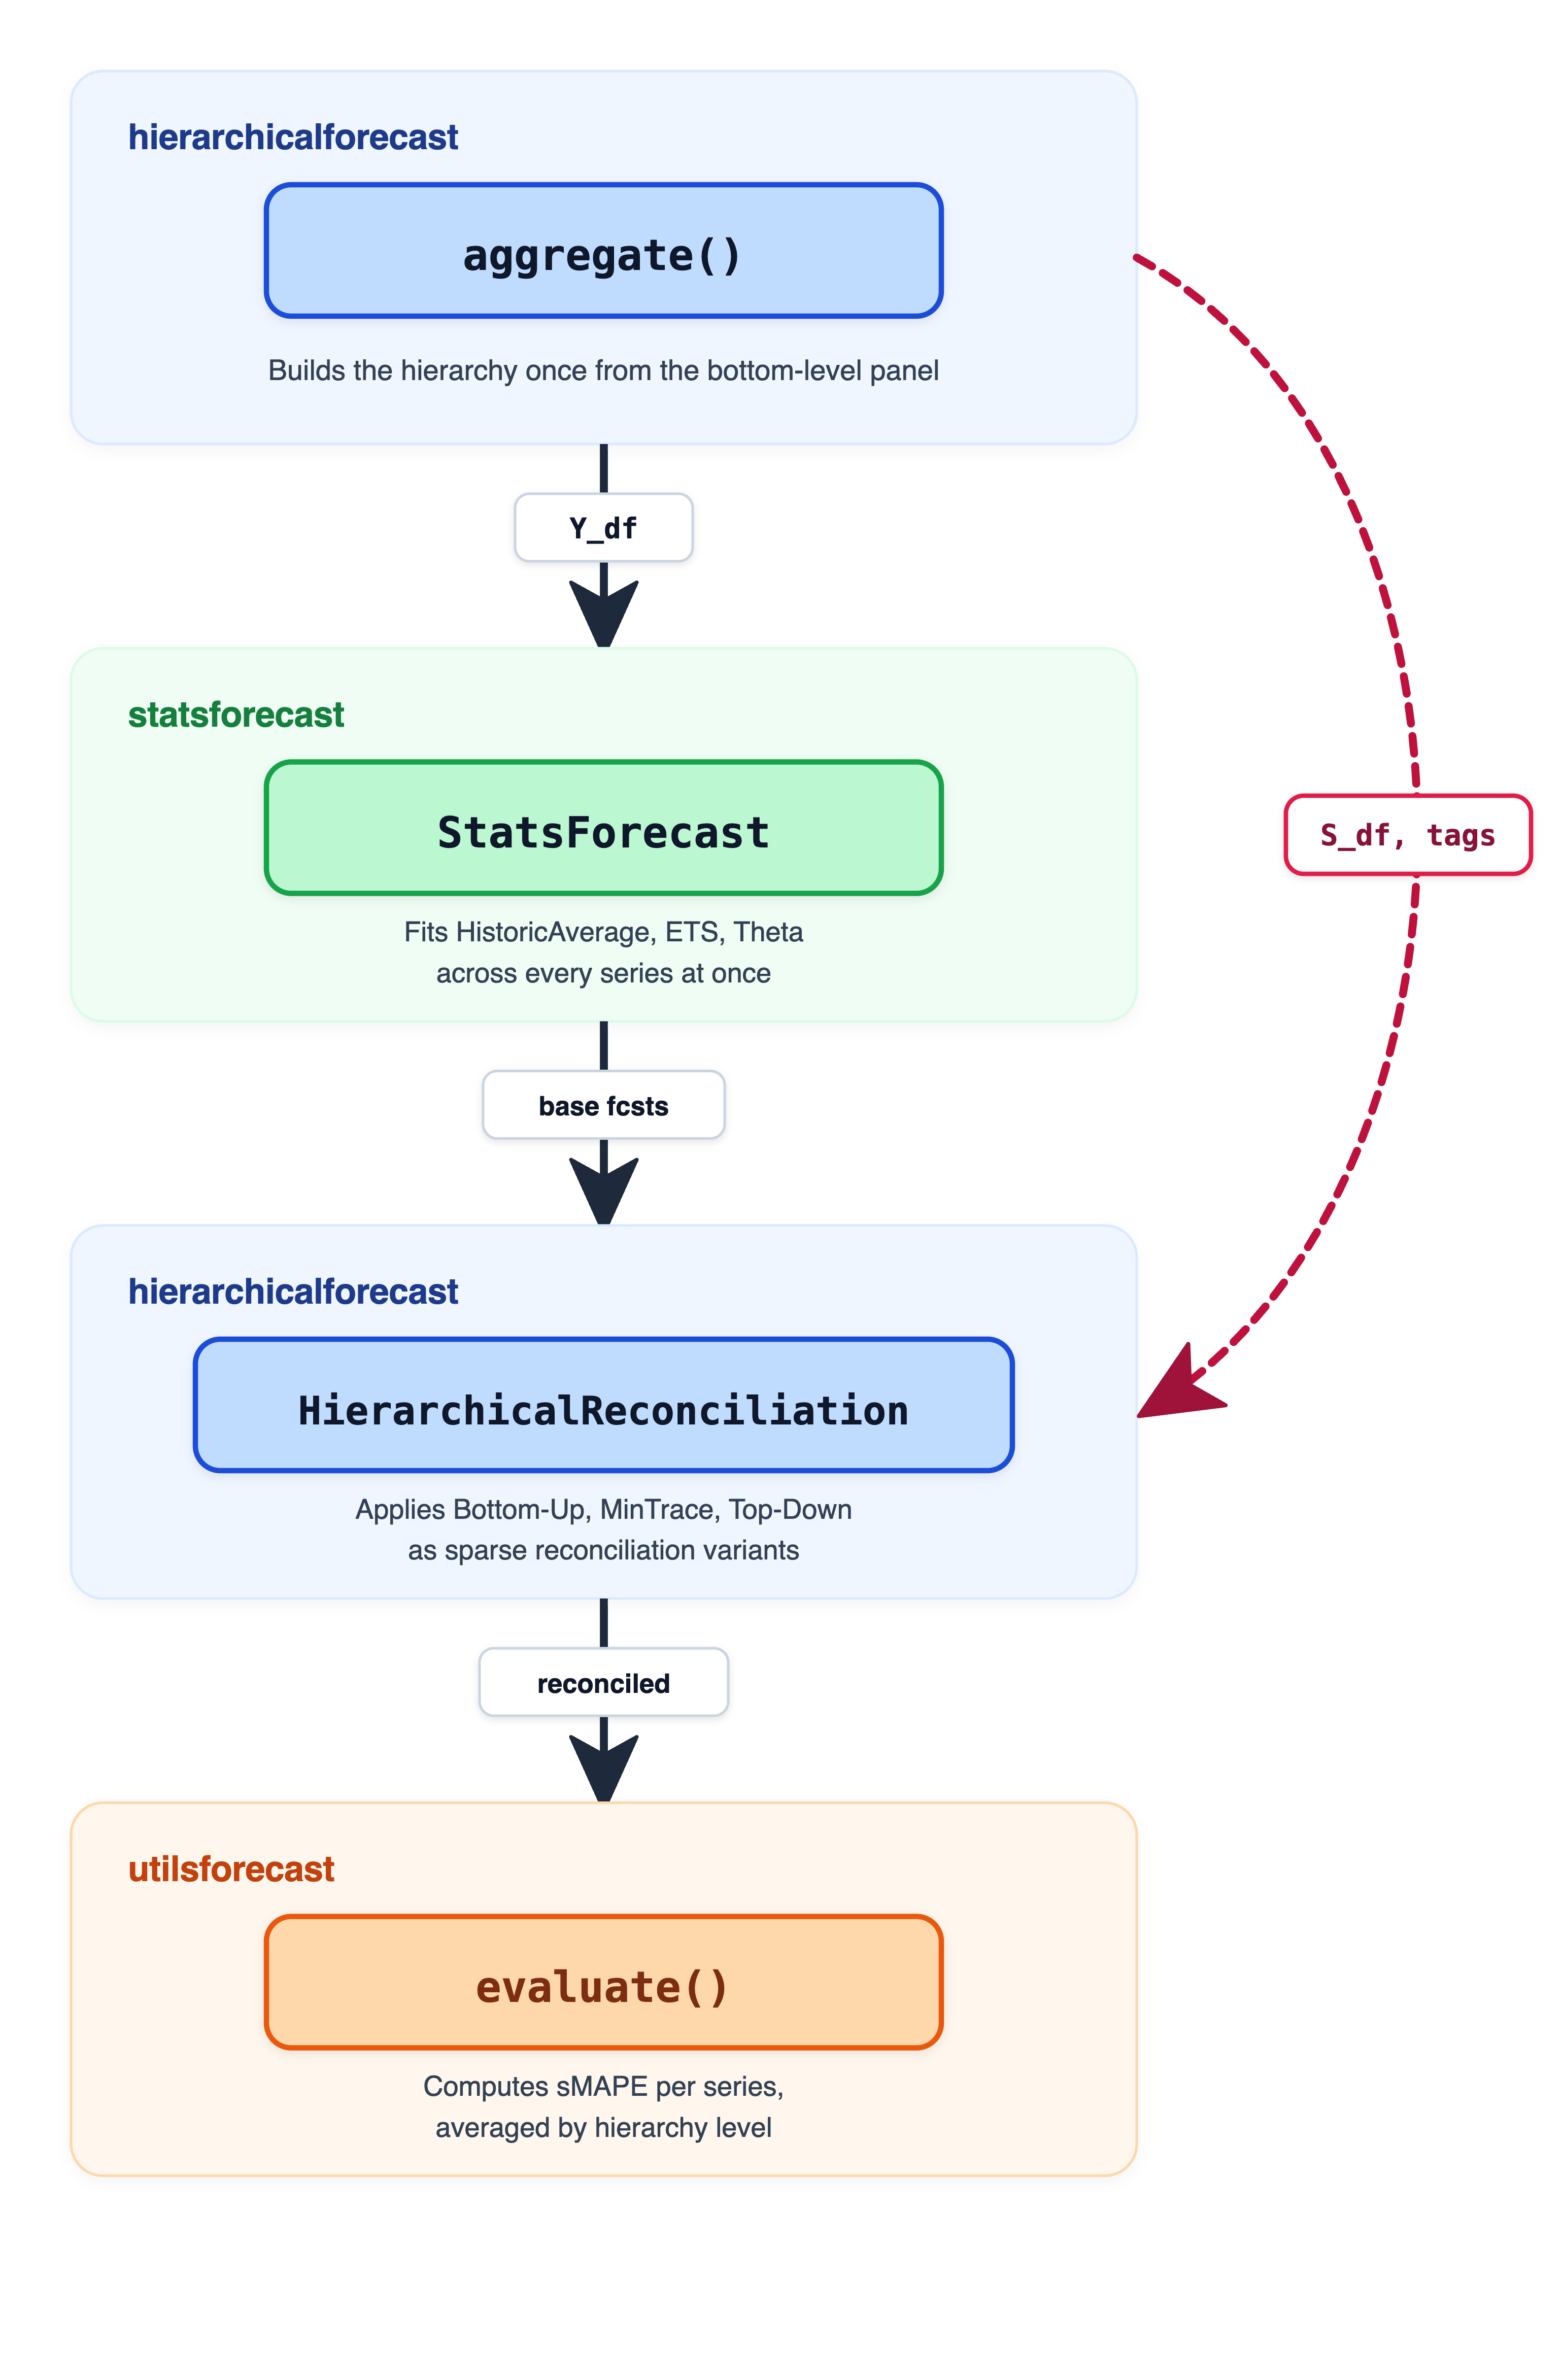
\includegraphics[width=1\linewidth]{Images/04DomainKnowledgeTools/toolDataFlow}
	\caption{Data objects passed between the three Nixtla libraries used in this thesis's forecasting pipeline.}\label{fig:toolDataFlow}
\end{figure}

\section{utilsforecast}
\label{sec:utilsforecastTool}

\texttt{utilsforecast} \cite{UtilsForecast:2026} supplies two things used throughout this thesis: the \texttt{smape} function, and a plotting helper.

The \texttt{smape} function is the single accuracy metric used everywhere in this thesis, and its exact formula, scaling convention, and zero/zero handling are presented once, in full, in Section~\ref{sec:evaluationFramework}, and are not repeated here. What belongs in this chapter is a reproducibility check rather than a definition: the pipeline notebook prints the library's own source code for \texttt{smape} alongside this thesis's independently written implementation, confirming that both compute the identical $|F-A| / (|F|+|A|)$ fraction with the same treatment of the zero/zero case, before the result is scaled to a percentage. Establishing this equivalence once, at the tooling level, means every sMAPE figure reported later in this thesis can be read as coming from a single, unambiguous formula rather than two conventions that merely look comparable.

The library's \texttt{plot\_series} function is a secondary tool used to overlay a series' actual history against its base and reconciled forecasts for visual inspection, as used in the pipeline's optional visualisation step.

\section{Supporting Stack}
\label{sec:supportingStackTool}

Several general-purpose libraries support the pipeline without being forecasting-specific themselves.

\textbf{pandas} \cite{McKinney:2010} and \textbf{NumPy} \cite{Harris:2020} handle every data-wrangling step outside of model fitting and reconciliation: reshaping the raw wide-format sales file (one row per item-store, one column per day) into long format, aggregating daily observations to monthly totals, and constructing the complete item-store-by-month grid that gives every series a value for every month, including months with zero sales.

\textbf{PyArrow} \cite{ApacheArrow:2026} provides Parquet support, used in two places for reproducibility. First, both the EDA and pipeline notebooks cache the raw M5 CSV files to Parquet after their first load, since Parquet is faster to re-read than re-parsing a CSV and preserves column data types (dates remain dates rather than becoming strings). Second, the pipeline's final step exports four Parquet files -- a hierarchy lookup table, the actual sales history, and the base and reconciled forecasts -- which are the sole data contract the Streamlit dashboard reads from (Chapter~\ref{chap:appDeployment}).

\textbf{Streamlit} \cite{Streamlit:2026} is the framework the dashboard (\texttt{app/streamlit\_app.py}) is built with, and the basis for its deployment on Streamlit Community Cloud. \textbf{Plotly} \cite{Plotly:2026} renders the dashboard's interactive charts and is also used as the plotting engine for \texttt{utilsforecast}'s \texttt{plot\_series} helper within the notebooks. For static exploratory plots that do not need to be interactive -- the histograms and bar charts in the EDA notebook -- \textbf{Matplotlib} \cite{Hunter:2007} is used instead.